\chapter{本科毕业论文文献综述}

\section{Word2Vec}
Word2Vec(Mikolov et al., 2013\cite{mikolov2013efficient})是一种表达词汇的方法,将一个单词用一个向量来表示,关系比较近的词(例如:king和queen,Shanghai和Beijing)在向量空间相对应的有比较近的距离。如何确定词的关系,一个朴素的想法就是在相似上下文中出现的单词关系比较近。
Word2Vec就是基于这一想法的一种高效的词汇表达方法。特别的,Word2Vec有两种算法,分别是Continuous Bag-of-Words(CBOW)和Skip-Gram。CBOW是根据环境词预测中心词,而Skip-Gram是根据中心词预测环境词。\\
\section{GloVe}
尽管Word2Vec已经被实验证明可以发掘出复杂的语义相似关系,但是是根据局部上下文来预测,往往忽略了整体的信息。与之对应的,Pennington et al.\cite{pennington2014glove}提出的Global Vectors for Word Representation (GloVe)使用全局的统计信息预测单词$i$出现在单词$j$的上下文中的概率。
具体来讲,GloVe使用最小二乘作为目标函数训练词词共生矩阵。GloVe在很多词汇相似性任务中已经表现出优越的结果。\\
\section{递归神经网络(RNN)}
递归神经网络是一种特别适合对时序信息建模的神经网络架构。在$t$时刻,RNN输入词矩阵$w_t$和上一步的隐式状态向量$h_{t-1}$进行下面的运算后,产生这一步点隐式状态向量:\\
\begin{equation}
h_t = f(Wx_t+Uh{t-1}+b)
\end{equation}
上式中$W$,$U$和$b$是这个RNN的参数。使用RNN对语段建模,能够提取到当前词的前面的所有词的信息考虑在内。
\section{GRU}
尽管RNN能够考虑时序关联信息,但是由于使用backpropagation进行优化目标函数时,求导产生的链式相乘,会导致,随着递归向前,产生权重指数级爆炸或消失的问题,难以捕捉长期时间关联。对于权重指数暴炸问题,可以简单的采用超出阈值后截断的方法,就能产生很好的结果。
而Chung et al.\cite{chung2015gated}Gated Recurrent Units(GRU)是一种激活单元,就是为了解决权重指数消失问题,对网络结构进行的优化。下面的一组公式表明了GRU如何根据$h_{t-1}$和$x_t$产生$h_{t}$:\\
\begin{equation}
z_t = \sigma (W^{(z)}x_i + U^{(z)}h_{t-1})
\end{equation}
\begin{equation}
r_t = \sigma (W^{(r)}x_i + U^{(r)}h_{t-1})
\end{equation}
\begin{equation}
\widetilde{h}_t = tanh(r_t \odot Uh_{t-1} + Wx_t)
\end{equation}
\begin{equation}
h_t = (1-z_t) \odot \widetilde{h}_t + z_t \odot h_{t-1}
\end{equation}
式(2)确定了$h_{t-1}$应该多大程度被带入下一阶段。式(3)表明$h_{t-1}$多大程度上影响$\widetilde{h}_t$。式(4)表明新的记忆$\widetilde{h}_t$是由输入$x_t$和$h_{t-1}$确定的。
式(5)表明隐式状态$h_t$最终是由以前的隐式状态$h_{t-1}$和$\widetilde{h}_t$新的记忆组成的。
\subsection{LSTM}
Long Short Term Memories(LSTM)\cite{hochreiter1997long}是另一种与GRU相似的激活单元,与GRU起到的作用相同。下面一组式子表明了LSTM的数学结构:\\
\begin{equation}
i_t = \sigma (W^{(i)}x_t + U^{(i)}h_{t-1})
\end{equation}
\begin{equation}
f_t = \sigma (W^{(f)}x_t + U^{(f)}h_{t-1})
\end{equation}
\begin{equation}
o_t = \sigma (W^{(o)}x_t + U^{(o)}h_{t-1})
\end{equation}
\begin{equation}
\widetilde{c}_t = tanh(W^{(c)}x_t + U^{(c)}h_{t-1})
\end{equation}
\begin{equation}
c_t = f_t \odot c_{t-1} + i_t \odot \widetilde{c}_t
\end{equation}
\begin{equation}
h_t = o_t \odot tanh(c_t)
\end{equation}
式(6)使用输入词和之前的隐式状态来判断输入词是否值得保存,用来产生新记忆。式(7)用来评估过去的记忆是否对于计算现在的记忆有用。
式(8)确定了最终记忆应该多大程度上保存到隐式状态中。式(9)根据输入词$x_t$和$h_{t-1}$产生新的记忆。式(10)根据新记忆和$h_{t-1}$产生最终记忆。
\section{Attention机制}
一句话中的不同的单词的重要性是不同的,例如名词、动词在就会比定冠词介词表达更多的意思。Bahdanau et al\cite{Bahdanauetal.2014}注意到了使用单向量的RNN的最终状态没有办法很好的表征不同输入的部分有不同重要性这一特征。
更近一步的,输出的不同部分可能更看重输入的特定部分。例如,在翻译中,输出的前几个单词通常是根据输入的前几个单词,而输出的后几个单词则更多的依赖于输入的后几个单词。\\
针对这一特点,Attention机制在编码的每一步,首先观察整个输入序列,然后决定在这一个阶段,哪一部分比较重要。\\
Bahdanau et al.提出的模型主要分成两个部分,编码部分和解码部分。编码部分对输入序列编码为向量,解码部分提取编码信息解码成语句,输出语句有一系列单词组成$y_1,...,y_m$。
\subsection{编码器}
令$(h_1,...,h_n)$为每个输入句子的隐式向量,这些向量可以使用GRU或者LSTM来产生,包含了词在上下文中的表达信息。
\subsection{解码器}
我们可以通过下面的递归式计算隐式状态$s_i$
\begin{equation}
s_i = f(s_{i-1},y_{i_1},c_i)
\end{equation}
在这里$s_{i-1}$是前一个隐式状态,$y_1$是上一个输出单词,上下文向量$c_i$是在解码的第$i$步根据解码状态对原文全文信息等提取表示。\\
对于输入序列中的隐式向量,计算下式得到一个权重值
\begin{equation}
e_{i,j} = a(s_{i-1},h_j)
\end{equation}
上式中$a$可以是任何定义域是$R$的函数,上市会得到一系列值$e_{i,1},...,e_{i,n}$。使用softmax归一化
\begin{equation}
\alpha_{i,j} = \frac{exp(e_{i,j})}{\sum_{k=1}^nexp(e_{i,k})}
\end{equation}
最后对输入隐式序列加权后生成最终的上下文状态向量。
\begin{equation}
c_i = \sum_{j=1}{n}\alpha_{i,j}h_j
\end{equation}
直观的来讲,这个向量能够在第$i$步捕获原文的上下文信息。
\section{Dynamic Memory Network}
Kumar et al.\cite{DBLP:journals/corr/KumarISBEPOGS15} Dynamic Memory Network由四个模块组成,分别是:输入模块、片段记忆模块、问题模块、回答模块。整体的架构如图表所示。\\
\begin{figure}[h]
      \centering
        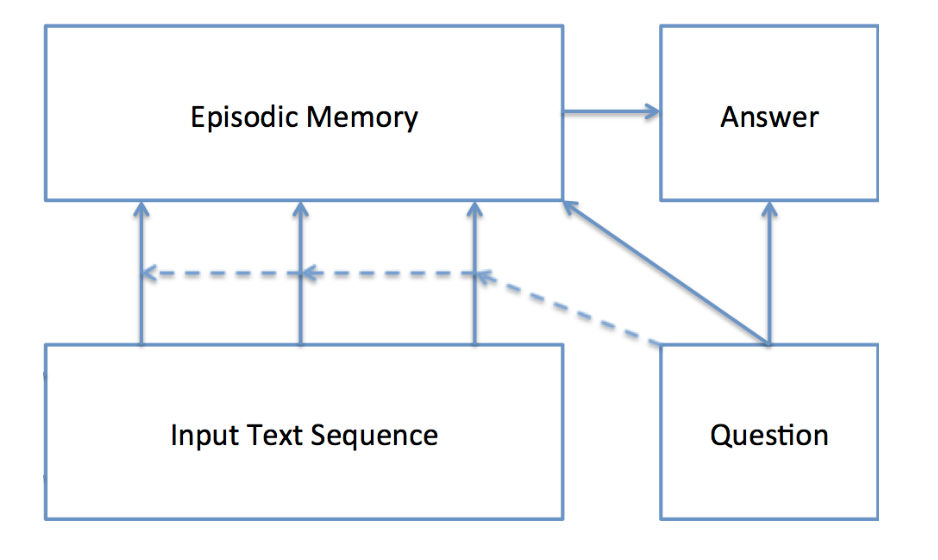
\includegraphics[width=0.6\textwidth]{./images/dynamic-memory-network-structure}
          \caption{Dynamic Memory Network模型架构}
      \end{figure} 
\subsection{输入模块}
输入模块接受一段文字,首先将文字中的每个单词转换为对应的词向量表示,然后将每个单词按顺序依次送入GRU。在每句话的结尾处,输出最终的隐式状态。
片段记忆模块将接收这些隐式状态,并进行总结推理。更加形式化的表示为,对于一个单词序列$T_I$ $w_1,...w_{T_I}$,我们根据下式来更新状态。\\
\begin{equation}
h_t = GRU(L[w_t],h_{t-1})
\end{equation}
然后对于由$T_I$作为子序列组成的序列$s_1,...s_{T_I}$,在每个子序列结束的时候,我们将最终的隐式状态$h_{s_1},...,h_{s_{T_I}}$输出
\subsection{问题模块}
问题模块与输入模块相似,接受问题作为输入,将问题序列中的每个单词转换为对应的词向量的表示,然后将每个词向量送入GRU,当所有问题单词都送入后,输出GRU的最终表示。
所以对于问题,形式化的表示为,对于一个包含单词$w_1,...,w_{T_Q}$的问题$T_Q$,我们使用下式更新隐式状态\\
\begin{equation}
h_t = GRU(L[w_t],h_{t-1})
\end{equation}
最后的输出为$h_{T_Q}$
\subsection{片段记忆模块}
片段记忆模块对于输入模块在每句话结束时输出的隐式状态和问题模块输出的隐式模块进行总结推理,产生一个最终记忆状态输出给回答模块,用于产生回答。\\
片段记忆模块主要由嵌套的两层GRU组成,内层GRU负责产生片段序列,外层GRU使用问题向量初始化后,根据片段序列产生最终记忆模块作为输入。\\
内层GRU每次通过遍历输入模块的输入序列产生一个片段,在每个片段结束后,内层GRU会把这个片段产生的最终状态送入外层GRU,下面的公式给出了内层GRU更新状态的方法:\cite{xiong2016dynamic}\\
\begin{equation}
z^i_t = [t_t,m,q,c_t \odot q, c_t \odot m,| c_t - q |,|c_t - m|]
\end{equation}
\begin{equation}
Z^i_t = W^{(2)}tanh(W^{(1)}z^i_t+b^{(1)})+b^{(2)}
\end{equation}
\begin{equation}
g^i_t = \frac{exp(Z^i_t)}{\sum_{k=1}^{M_i}exp(Z^i_k)}
\end{equation}
\begin{equation}
h^i_t = g^i_tGRU(c_t,h^i_{t-1} + (1 - g^i_t))h^i_{t-1}
\end{equation}
上面的式子中结合当前状态$c_t$,当前记忆状态$m$和记忆状态$q$来决定当前句子是否值得编码进入回答$g^i_t$中,如果$g^i_t \approx 0$,当前句子将被忽略,现在的状态即为之前的状态。
这个片段的最终状态是当内层GRU遍历晚所有句子之后产生的状态$e^i = h_{T_I}$\\
外层GRU将根据之前的记忆状态和本次片段状态来更新片段状态。\\
\begin{equation}
m^t = GRU(e^t,m^{t-1})
\end{equation}
外层GRU的最终记忆状态将被送入回答模块。
\begin{figure}[h]
      \centering
        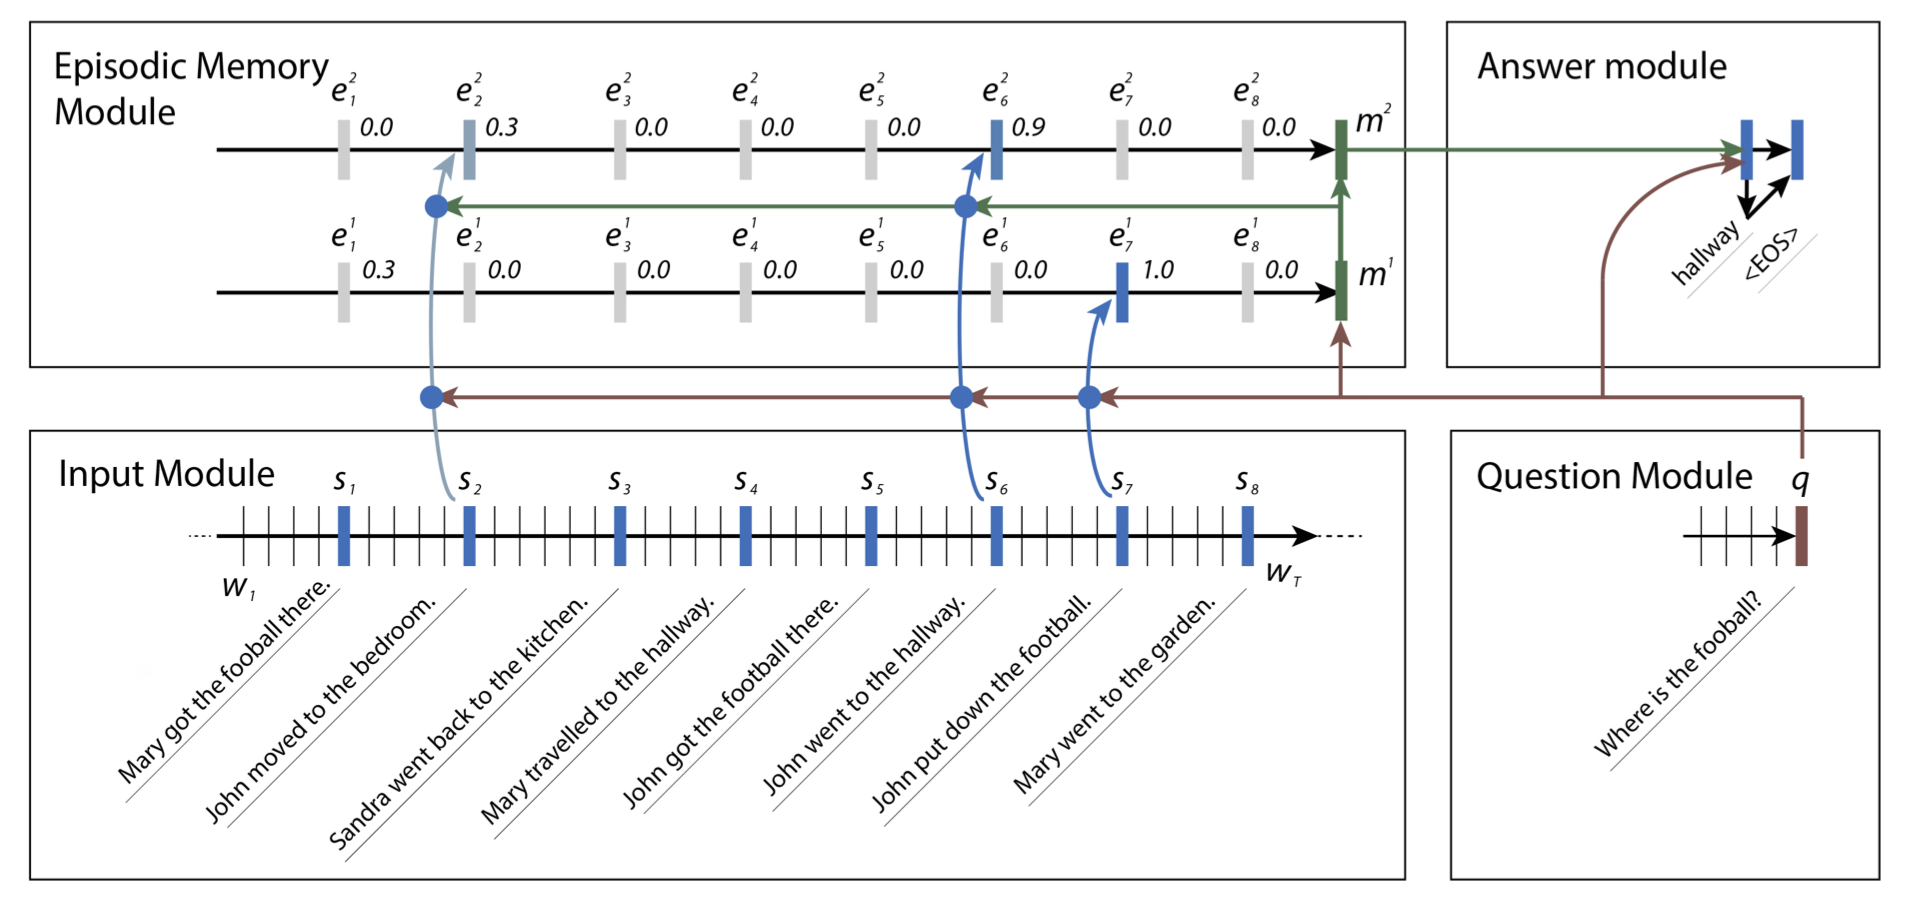
\includegraphics[width=0.9\textwidth]{./images/episodic-memory-structure}
          \caption{片段记忆模块架构}
      \end{figure}
\subsection{回答模块}
回答模块通过softmax产生对于回答标签的概率分布,然后产生单个单词回答,也可以将输入状态向量RNN来产生多个单词的回答。